%  LaTeX support: latex@mdpi.com 
%  For support, please attach all files needed for compiling as well as the log file, and specify your operating system, LaTeX version, and LaTeX editor.

%=================================================================
\documentclass[jimaging,article,submit,pdftex,moreauthors]{Definitions/mdpi} 

% Figures live at repository root; this manuscript is compiled from draft/.
\graphicspath{{../}}
%\documentclass[preprints,article,submit,pdftex,moreauthors]{Definitions/mdpi} 
% For posting an early version of this manuscript as a preprint, you may use "preprints" as the journal. Changing "submit" to "accept" before posting will remove line numbers.

% Below journals will use APA reference format:
% admsci, aieduc, behavsci, businesses, econometrics, economies, education, ejihpe, famsci, games, humans, ijcs, ijfs, jintelligence, journalmedia, jrfm, jsam, languages, peacestud, psycholint, publications, tourismhosp, youth

% Below journals will use Chicago reference format:
% arts, genealogy, histories, humanities, laws, literature, religions, risks, socsci

%--------------------
% Class Options:
%--------------------
%----------
% journal
%----------
% Choose between the following MDPI journals:
% accountaudit, acoustics, actuators, addictions, adhesives, admsci, adolescents, aerobiology, aerospace, agriculture, agriengineering, agrochemicals, agronomy, ai, aichem, aieduc, aieng, aimater, aimed, aipa, air, aisens, algorithms, allergies, alloys, amh, analog, analytica, analytics, anatomia, anesthres, animals, antibiotics, antibodies, antioxidants, applbiosci, appliedchem, appliedmath, appliedphys, applmech, applmicrobiol, applnano, applsci, aquacj, architecture, arm, arthropoda, arts, asc, asi, astronautics, astronomy, atmosphere, atoms, audiolres, automation, axioms, bacteria, batteries, bdcc, behavsci, beverages, biochem, bioengineering, biologics, biology, biomass, biomechanics, biomed, biomedicines, biomedinformatics, biomimetics, biomolecules, biophysica, bioresourbioprod, biosensors, biosphere, biotech, birds, blockchains, bloods, blsf, brainsci, breath, buildings, businesses, cancers, carbon, cardio, cardiogenetics, cardiovascmed, catalysts, cells, ceramics, challenges, chemengineering, chemistry, chemosensors, chemproc, children, chips, cimb, civileng, cleantechnol, climate, clinbioenerg, clinpract, clockssleep, cmd, cmtr, coasts, coatings, colloids, colorants, commodities, complexities, complications, compounds, computation, computers, condensedmatter, conservation, constrmater, cosmetics, covid, crops, cryo, cryptography, crystals, csmf, ctn, culture, curroncol, cyber, dairy, data, ddc, dentistry, dermato, dermatopathology, designs, devices, dhi, diabetology, diagnostics, dietetics, digital, disabilities, diseases, diversity, dna, drones, dynamics, earth, ebj, ecm, ecologies, econometrics, economies, edm, education, eesp, ejihpe, electricity, electrochem, electronicmat, electronics, encyclopedia, endocrines, energies, eng, engproc, entomology, entropy, environments, environremediat, epidemiologia, epigenomes, esa, est, famsci, fermentation, fibers, fintech, fire, fishes, fluids, foods, forecasting, forensicsci, forests, fossstud, foundations, fractalfract, fuels, future, futureinternet, futurepharmacol, futurephys, futuretransp, galaxies, games, gases, gastroent, gastrointestdisord, gastronomy, gels, genealogy, genes, geographies, geohazards, geomatics, geometry, geosciences, geotechnics, geriatrics, germs, glacies, grasses, green, greenhealth, gucdd, hardware, hazardousmatters, healthcare, hearts, hemato, hematolrep, hep, heritage, higheredu, highthroughput, histories, horticulturae, hospitals, humanities, humans, hydrobiology, hydrogen, hydrology, hydropower, hygiene, idr, iic, ijcs, ijem, ijerph, ijfs, ijgi, ijmd, ijms, ijns, ijom, ijpb, ijt, ijtm, ijtpp, ime, immuno, informatics, information, infrastructures, inorganics, insects, instruments, inventions, iot, j, jaestheticmed, jal, jcdd, jcm, jcp, jcrm, jcs, jcto, jdad, jdb, jdream, jemr, jeta, jfb, jfmk, jgbg, jgg, jimaging, jintelligence, jlpea, jmahp, jmmp, jmms, jmp, jmse, jne, jnt, jof, joi, joitmc, joma, jop, joptm, jor, journalmedia, jox, jpbi, jphytomed, jpm, jrfm, jsam, jsan, jtaer, jvd, jzbg, kidneydial, kinasesphosphatases, knowledge, labmed, laboratories, lae, land, languages, laws, life, lights, limnolrev, lipidology, liquids, literature, livers, logics, logistics, lubricants, lymphatics, machines, macromol, magnetism, magnetochemistry, make, marinedrugs, materials, materproc, mathematics, mca, measurements, medicina, medicines, medsci, membranes, merits, metabolites, metals, meteorology, methane, metrics, metrology, micro, microarrays, microbiolres, microelectronics, micromachines, microorganisms, microplastics, microwave, minerals, mining, mmphys, modelling, molbank, molecules, mps, msf, mti, multimedia, muscles, nanoenergyadv, nanomanufacturing, nanomaterials, ncrna, ndt, network, neuroglia, neuroimaging, neurolint, neurosci, nitrogen, notspecified, nursrep, nutraceuticals, nutrients, obesities, occuphealth, oceans, ohbm, onco, optics, oral, organics, organoids, osteology, oxygen, pandemics, parasites, parasitologia, particles, pathogens, pathophysiology, peacestud, pediatrrep, pets, pharmaceuticals, pharmaceutics, pharmacoepidemiology, pharmacy, philosophies, photochem, photonics, phycology, physchem, physics, physiologia, plants, plasma, platforms, pollutants, polymers, polysaccharides, populations, poultry, powders, precipitation, precisoncol, preprints, proceedings, processes, prosthesis, proteomes, psf, psychiatryint, psychoactives, psycholint, publications, purification, quantumrep, quaternary, qubs, radiation, rdt, reactions, realestate, receptors, recycling, regeneration, religions, remotesensing, reports, reprodmed, resources, rheumato, risks, rjpm, robotics, rsee, ruminants, safety, sci, scipharm, sclerosis, seeds, sensors, separations, sexes, shi, signals, sinusitis, siuj, skins, smartcities, sna, societies, socsci, software, soilsystems, solar, solids, spectroscj, sports, standards, stats, std, stratsediment, stresses, surfaces, surgeries, suschem, sustainability, symmetry, synbio, systems, tae, targets, taxonomy, technologies, telecom, test, textiles, thalassrep, therapeutics, thermo, timespace, tomography, tourismhosp, toxics, toxins, tph, transplantology, transportation, traumacare, traumas, tri, tropicalmed, universe, urbansci, uro, vaccines, vehicles, venereology, vetsci, vibration, virtualworlds, viruses, vision, waste, water, welding, wem, wevj, wild, wind, women, world, youth, zoonoticdis

%---------
% article
%---------
% The default type of manuscript is "article", but can be replaced by: 
% abstract, addendum, article, benchmark, book, bookreview, briefcommunication, briefreport, casereport, changes, clinicopathologicalchallenge, comment, commentary, communication, conceptpaper, conferenceproceedings, correction, conferencereport, creative, datadescriptor, discussion, entry, expressionofconcern, extendedabstract, editorial, essay, erratum, fieldguide, hypothesis, interestingimages, letter, meetingreport, monograph, newbookreceived, obituary, opinion, proceedingpaper, projectreport, reply, retraction, review, perspective, protocol, shortnote, studyprotocol, supfile, systematicreview, technicalnote, viewpoint, guidelines, registeredreport, tutorial,  giantsinurology, urologyaroundtheworld
% supfile = supplementary materials

%----------
% submit
%----------
% The class option "submit" will be changed to "accept" by the Editorial Office when the paper is accepted. This will only make changes to the frontpage (e.g., the logo of the journal will get visible), the headings, and the copyright information. Also, line numbering will be removed. Journal info and pagination for accepted papers will also be assigned by the Editorial Office.

%------------------
% moreauthors
%------------------
% If there is only one author the class option oneauthor should be used. Otherwise use the class option moreauthors.

%---------
% pdftex
%---------
% The option pdftex is for use with pdfLaTeX. Remove "pdftex" for (1) compiling with LaTeX & dvi2pdf (if eps figures are used) or for (2) compiling with XeLaTeX.

%=================================================================
% MDPI internal commands - do not modify
\firstpage{1} 
\makeatletter 
\setcounter{page}{\@firstpage} 
\makeatother
\pubvolume{1}
\issuenum{1}
\articlenumber{0}
\pubyear{2026}
\copyrightyear{2026}
%\externaleditor{Firstname Lastname} % More than 1 editor, please add `` and '' before the last editor name
\datereceived{ } 
\daterevised{ } % Comment out if no revised date
\dateaccepted{ } 
\datepublished{ } 
%\datecorrected{} % For corrected papers: "Corrected: XXX" date in the original paper.
%\dateretracted{} % For retracted papers: "Retracted: XXX" date in the original paper.
%\doinum{} % Used for some special journals, like molbank
%\pdfoutput=1 % Uncommented for upload to arXiv.org
%\CorrStatement{yes}  % For updates
%\longauthorlist{yes} % For many authors that exceed the left citation part
%\IsAssociation{yes} % For association journals

%=================================================================
% Add packages and commands here. The following packages are loaded in our class file: fontenc, inputenc, calc, indentfirst, fancyhdr, graphicx, epstopdf, lastpage, ifthen, float, amsmath, amssymb, lineno, setspace, enumitem, mathpazo, booktabs, titlesec, etoolbox, tabto, xcolor, colortbl, soul, multirow, microtype, tikz, totcount, changepage, attrib, upgreek, array, tabularx, pbox, ragged2e, tocloft, marginnote, marginfix, enotez, amsthm, natbib, hyperref, cleveref, scrextend, url, geometry, newfloat, caption, draftwatermark, seqsplit
% cleveref: load \crefname definitions after \begin{document}

%=================================================================
% Please use the following mathematics environments: Theorem, Lemma, Corollary, Proposition, Characterization, Property, Problem, Example, ExamplesandDefinitions, Hypothesis, Remark, Definition, Notation, Assumption
%% For proofs, please use the proof environment (the amsthm package is loaded by the MDPI class).

%=================================================================
% Full title of the paper (Capitalized)
\Title{HER-TransMorph: Topology-Preserving Transformer-Based Deformable Brain MRI Registration with Hyperelastic Regularization}
% PH = pending Stage B value (greppable placeholder token)
\providecommand{\PH}[1]{\textcolor{red}{\textbf{[#1]}}}

% Author Orchid ID: enter ID or remove command
\newcommand{\orcidauthorA}{0000-0000-0000-000X} % Add \orcidA{} behind the author's name
%\newcommand{\orcidauthorB}{0000-0000-0000-000X} % Add \orcidB{} behind the author's name

% Authors, for the paper (add full first names)
\Author{Author One $^{1}$\orcidA{}, Author Two $^{2}$ and Corresponding Author $^{2,}$*}

%\longauthorlist{yes}

% MDPI internal command: Authors, for metadata in PDF
\AuthorNames{Author One, Author Two and Corresponding Author}

%\longauthorlist{yes}

% Affiliations / Addresses (Add [1] after \address if there is only one affiliation.)
\address{%
$^{1}$ \quad Department of Biomedical Engineering, Institution One, City, Country; author1@example.edu\\
$^{2}$ \quad Department of Medical Imaging, Institution Two, City, Country; author2@example.edu}

% Contact information of the corresponding author
\corres{Correspondence: corresponding.author@example.edu; Tel.: +00-000000000}

% Current address and/or shared authorship
%\firstnote{Current address: Affiliation.}  
% Current address should not be the same as any items in the Affiliation section.

%\secondnote{These authors contributed equally to this work.}
% The commands \thirdnote{} till \eighthnote{} are available for further notes.

%\simplesumm{} % Simple summary

%\conference{} % An extended version of a conference paper

% Abstract (Do not insert blank lines, i.e. \\) 
\abstract{Background: Deformable brain MRI registration requires preserving deformation topology in addition to overlap accuracy. Methods: HER-TransMorph augments a TransMorph backbone with hyperelastic regularization terms targeting volume-change moderation and anti-folding control, while keeping the same unsupervised objective family across datasets. We evaluate the method on two complementary protocols---IXI atlas-to-subject and OASIS inter-subject---against learning-based and classical baselines, and report paired Wilcoxon signed-rank tests with Benjamini--Hochberg FDR correction where available. Results: HER-TransMorph maintains competitive overlap (IXI Dice: 0.7537 \(\pm\) 0.0275; OASIS Dice: \PH{OASIS Dice mean±std}) while reducing topology violations (IXI non-positive Jacobian ratio: 0.0000 vs.\ 0.0153 for TransMorph; OASIS: \PH{HER non\_jac OASIS} vs.\ \PH{TM non\_jac OASIS}, q < \PH{q OASIS non\_jac}) and improving Jacobian regularity (IXI SDlogJ: 0.3280 vs.\ 0.4920; OASIS SDlogJ: \PH{HER SDlogJ OASIS} vs.\ \PH{TM SDlogJ OASIS}). Conclusions: HER-TransMorph yields topology-preserving deformations across complementary registration regimes, supporting downstream Jacobian-based morphometric analysis.}

% Keywords
\keyword{medical image registration; deformable registration; transformer; hyperelastic regularization; topology preservation; diffeomorphism; Jacobian determinant; brain MRI}

% The fields PACS, MSC, and JEL may be left empty or commented out if not applicable
%\PACS{J0101}
%\MSC{}
%\JEL{}

%%%%%%%%%%%%%%%%%%%%%%%%%%%%%%%%%%%%%%%%%%
% Only for the journal Diversity
%\LSID{\url{http://}}

%%%%%%%%%%%%%%%%%%%%%%%%%%%%%%%%%%%%%%%%%%
% Only for the journal Applied Sciences
%\featuredapplication{Authors are encouraged to provide a concise description of the specific application or a potential application of the work. This section is not mandatory.}
%%%%%%%%%%%%%%%%%%%%%%%%%%%%%%%%%%%%%%%%%%

%%%%%%%%%%%%%%%%%%%%%%%%%%%%%%%%%%%%%%%%%%
% Only for the journal Data
%\dataset{DOI number or link to the deposited data set if the data set is published separately. If the data set shall be published as a supplement to this paper, this field will be filled by the journal editors. In this case, please submit the data set as a supplement.}
%\datasetlicense{License under which the data set is made available (CC0, CC-BY, CC-BY-SA, CC-BY-NC, etc.)}

%%%%%%%%%%%%%%%%%%%%%%%%%%%%%%%%%%%%%%%%%%
% Only for the journal BioTech, Fishes, Neuroimaging and Toxins
%\keycontribution{The breakthroughs or highlights of the manuscript. Authors can write one or two sentences to describe the most important part of the paper.}

%%%%%%%%%%%%%%%%%%%%%%%%%%%%%%%%%%%%%%%%%%
% Only for the journal Encyclopedia
%\encyclopediadef{For entry manuscripts only: please provide a brief overview of the entry title instead of an abstract.}

%%%%%%%%%%%%%%%%%%%%%%%%%%%%%%%%%%%%%%%%%%
% Different journals have different requirements. Please check the specific journal guidelines in the "Instructions for Authors" on the journal's official website.
%\addhighlights{yes}
%\renewcommand{\addhighlights}{%
%
%\noindent The goal is to increase the discoverability and readability of the article via search engines and other scholars. Highlights should not be a copy of the abstract, but a simple text allowing the reader to quickly and simplified find out what the article is about and what can be cited from it. Each of these parts should be devoted up to 2~bullet points.\vspace{3pt}\\
%\textbf{What are the main findings?}
% \begin{itemize}[labelsep=2.5mm,topsep=-3pt]
% \item First bullet.
% \item Second bullet.
% \end{itemize}\vspace{3pt}
%\textbf{What are the implications of the main findings?}
% \begin{itemize}[labelsep=2.5mm,topsep=-3pt]
% \item First bullet.
% \item Second bullet.
% \end{itemize}
%}

%%%%%%%%%%%%%%%%%%%%%%%%%%%%%%%%%%%%%%%%%%
\begin{document}

%%%%%%%%%%%%%%%%%%%%%%%%%%%%%%%%%%%%%%%%%%
\section{Introduction}

Deformable registration is a central component of computational neuroimaging pipelines, including atlas propagation, longitudinal analysis, and voxel-wise morphometry. In recent years, learning-based methods have significantly reduced inference time compared with classical iterative optimization \citep{balakrishnan2019voxelmorph,kim2021cyclemorph}. However, high overlap metrics alone are not sufficient when deformation fields contain local foldings or implausible volume changes.

Transformer-based registration improves long-range contextual modeling and has shown strong performance on 3D MRI tasks \citep{chen2022transmorph}. Nevertheless, unconstrained displacement prediction may still produce non-diffeomorphic regions, which can invalidate downstream Jacobian-based analysis. To address this, we integrate a Hyperelastic Regularization (HER)\footnote{Throughout this manuscript, HER denotes Hyperelastic Regularization and is unrelated to the Human Epidermal Growth Factor Receptor (HER2) acronym in oncology.} formulation into a TransMorph backbone and explicitly optimize deformation plausibility.

This manuscript targets Journal of Imaging with an imaging-methodology contribution focused on topology preservation and regular deformation behavior. We emphasize physically plausible transformations while maintaining competitive registration accuracy.

The contributions of this study are:
\begin{itemize}
\item A hyperelastic-regularized Transformer registration framework (HER-TransMorph) that combines similarity, smoothness, and a two-term hyperelastic regularizer (volume-change and anti-folding) in a unified objective;
\item A full baseline comparison under a unified IXI protocol including deep-learning models and classical affine/SyN methods;
\item Subject-level paired statistical validation (Wilcoxon + BH-FDR), with dual-protocol evaluation across IXI and OASIS (\PH{OASIS stats pending Stage B}), to test robustness of topology-preserving behavior.
\end{itemize}

\section{Related Work}

\subsection{DL-Based Registration}
Learning-based registration, represented by VoxelMorph and its descendants, enables fast inference with strong overlap quality \citep{balakrishnan2019voxelmorph}. Subsequent CNN and hybrid variants (e.g., CycleMorph and MIDIR) improve architectural capacity \citep{kim2021cyclemorph,qiu2021midir}, but deformation plausibility can degrade when the objective is dominated by image similarity terms.

\subsection{Topology Preservation and Regularization}
Topology-aware constraints are central for anatomically meaningful deformation fields. Jacobian-aware regularization and hyperelastic formulations explicitly penalize implausible local volume changes, discontinuities, and folding patterns \citep{burger2013hyperelastic,ashburner1999morphometry,rueckert1999nonrigid}. These constraints are especially relevant when registration outputs are used for morphometric analysis.

\subsection{Transformer-Based Efficient Registration}
Transformer backbones improve long-range context aggregation in volumetric registration and have become competitive baselines \citep{chen2022transmorph,liu2021swin}. Recent Transformer-family methods (including CoTr, nnFormer, PVT, and ViTVNet) broaden architectural design space \citep{xie2021cotr,zhou2021nnformer,wang2021pvt,vitvnet2021}, but explicit regularization is still required to stabilize topology while preserving alignment accuracy.

%%%%%%%%%%%%%%%%%%%%%%%%%%%%%%%%%%%%%%%%%%
\section{Materials and Methods}

\subsection{Dataset and Preprocessing}
Experiments are conducted on the IXI dataset \citep{ixidataset} with an atlas-to-subject registration protocol. The dataset split is 403/58/115 (train/validation/test), and all test results reported in this manuscript are based on 115 held-out subjects. Preprocessing includes skull/field handling as implemented in the repository pipeline, spatial normalization to a common template space, and cropping/resampling to \(160 \times 192 \times 224\). The fixed atlas for the IXI atlas-to-subject protocol is \texttt{IXI\_data/atlas.pkl}, consistent with the atlas distributed in the TransMorph codebase \citep{chen2022transmorph,kim2021cyclemorph}.

To assess generalization beyond IXI atlas-to-subject, we additionally evaluate on OASIS using the inter-subject registration protocol established by MICCAI Learn2Reg Task 03 \citep{hering2022learn2reg}. We use the neurite-OASIS preprocessed release \citep{hoopes2022hypermorph}: 414 T1w volumes affinely aligned to FreeSurfer Talairach space at \(160\times192\times224\), with 35-label FreeSurfer segmentations. Test pairs follow the official Learn2Reg validation pairing released as \texttt{pairs\_val.csv} (\PH{N\_OASIS pairs}). Following common practice \citep{chen2022transmorph,hoopes2022hypermorph}, OASIS is evaluated inter-subject (no canonical fixed atlas), while IXI retains atlas-to-subject evaluation.

\begin{table}[H]
\caption{Dataset and experimental setup summary.\label{tab1}}
\begin{tabularx}{\textwidth}{lX}
\toprule
\textbf{Item} & \textbf{Configuration} \\
\midrule
Dataset & IXI T1 MRI, atlas-to-subject registration protocol \\
Split & 403 / 58 / 115 (train / validation / test) \\
Input shape & \(160 \times 192 \times 224\) (cropped/resampled template space) \\
Label protocol & Grouped Dice over 17 bilateral/related VOI groups (\texttt{analysis\_trans.py} / \texttt{IXI/analysis.py}) \\
Compared families & TransMorph family, CNN/hybrid baselines, and classical Affine/SyN \\
Checkpoint source & Repository checkpoints configured in \texttt{IXI/eval\_configs.yaml} and per-model manifests \\
\bottomrule
\end{tabularx}
\end{table}

\subsection{Baseline Model}
The base architecture is TransMorph, a Transformer-based dense deformable registration network with a Swin-style encoder and decoder-to-flow prediction head \citep{chen2022transmorph,liu2021swin}. We compare HER-TransMorph against deep-learning and classical baselines under identical preprocessing and evaluation scripts:
\begin{itemize}
\item Transformer family: TransMorph, TransMorphBayes, CoTr, nnFormer;
\item CNN / hybrid baselines: VoxelMorph-1, CycleMorph, MIDIR;
\item Classical baselines: affine (MI-based) and SyN (ANTs).
\end{itemize}
Checkpoint and version identifiers are documented in the repository evaluation configuration and the supplementary checkpoint manifest.
Published baseline checkpoints were obtained from official TransMorph-related repositories and are assumed not to have seen the 115-subject IXI test split during their original training, following the protocol reporting style of \citet{chen2022transmorph}. Where this cannot be verified from upstream model cards, this assumption is stated explicitly.

\subsection{Proposed HER Method}
HER-TransMorph augments the TransMorph baseline with explicit hyperelastic regularization to constrain unrealistic local distortion. The operating-point regularizer targets two complementary aspects of deformation quality: volume-change moderation and anti-folding behavior near singular Jacobian regions. A length-change term is retained in the general mathematical formulation but its coefficient is set to zero in the final operating point because \(\mathcal{L}_{\mathrm{grad}}\) already constrains displacement smoothness and length-change behavior.

\subsection{Loss Function}
The training objective is
\begin{linenomath}
\begin{equation}
\mathcal{L} = \mathcal{L}_{\mathrm{NCC}} + \lambda_{\mathrm{grad}}\mathcal{L}_{\mathrm{grad}} + \lambda_{\mathrm{HER}}\mathcal{L}_{\mathrm{HER}}.
\end{equation}
\end{linenomath}
Let \(u:\Omega\to\mathbb{R}^3\) denote the displacement field over image domain \(\Omega\), \(\varphi=\mathrm{Id}+u\) the transformation, and \(J_{\varphi}(x)=\mathrm{I}+\nabla u(x)\) the Jacobian matrix. The hyperelastic term is
\begin{linenomath}
\begin{equation}
\mathcal{L}_{\mathrm{HER}} = \alpha \, \mathcal{L}_{\mathrm{length}} + \beta \, \mathcal{L}_{\mathrm{volume}} + \gamma \, \mathcal{L}_{\mathrm{fold}}.
\end{equation}
\end{linenomath}
\begin{linenomath}
\begin{equation}
\mathcal{L}_{\mathrm{length}}(u)=\frac{1}{|\Omega|}\sum_{x\in\Omega}\|\nabla u(x)\|_F^2,
\end{equation}
\end{linenomath}
\begin{linenomath}
\begin{equation}
\mathcal{L}_{\mathrm{volume}}(\varphi)=\frac{1}{|\Omega|}\sum_{x\in\Omega}\frac{(\det J_{\varphi}(x)-1)^2}{\max(\det J_{\varphi}(x),\epsilon)},
\end{equation}
\end{linenomath}
\begin{linenomath}
\begin{equation}
\mathcal{L}_{\mathrm{fold}}(\varphi)=\frac{1}{|\Omega|}\sum_{x\in\Omega}\left[\max(0,\epsilon-\det J_{\varphi}(x))\right]^2.
\end{equation}
\end{linenomath}
The rational volume form follows the hyperelastic formulation in \citet{burger2013hyperelastic}; compared with a plain quadratic \((\det J-1)^2\), it penalizes compressive (small-\(\det J\)) deformations more strongly. Final hyperparameters are:
\[
\lambda_{\mathrm{grad}} = 1.0, \quad
\lambda_{\mathrm{HER}} = 1.0, \quad
\alpha = 0, \quad
\beta = 0.02, \quad
\gamma = 20, \quad
\epsilon = 10^{-3}.
\]
In the final operating point, \(\alpha=0\) is intentional: \(\mathcal{L}_{\mathrm{grad}}\) already controls length-change behavior, while \(\beta\) and \(\gamma\) dominate topology-oriented regularization.

\subsection{Training Details}
Training settings for HER-TransMorph are: optimizer Adam \citep{kingma2014adam}, learning rate \(1\times10^{-4}\), batch size 2, and 500 epochs. Hardware for the current runs is NVIDIA RTX PRO 6000 Blackwell Workstation Edition (97,887 MiB VRAM), CUDA 12.8, and PyTorch 2.12.0.dev20260408+cu128. Baseline models are evaluated using published/repository checkpoints under the same test protocol (see \texttt{IXI/eval\_configs.yaml}); classical baselines use ANTs/ANTsPy and SimpleITK implementations \citep{avants2008ants,antspyx2024,simpleitk2013}. A stable-release reproducibility check on PyTorch 2.5.x is planned for the final submission package (\PH{stable-version verification pending Stage B}).

\subsection{Evaluation Metrics}
Primary evaluation metrics include Dice, Jaccard, HD95, ASSD, and NSD@1 mm \citep{dice1945,heimann2009,nikolov2018}. Deformation regularity is assessed by non-positive Jacobian ratio, SDlogJ, Jacobian quantiles (\(J_{\min}, J_{p01}, J_{p50}, J_{p99}, J_{\max}\)), bending energy, and mean absolute divergence \citep{rueckert1999nonrigid,ashburner1999morphometry}. Intensity-based metrics (NCC, LNCC, MI, NMI, SSIM, PSNR) and runtime/memory observations are reported in the Supplementary Materials.

\subsection{Statistical Analysis}
For each metric, HER-TransMorph is compared with each baseline using paired Wilcoxon signed-rank tests over the test subjects \citep{wilcoxon1945}. Multiple comparisons are corrected using Benjamini--Hochberg FDR \citep{bh1995}. Statistical significance is defined as q < 0.05. For metrics where higher is better (e.g., Dice), directionality is interpreted accordingly.

%%%%%%%%%%%%%%%%%%%%%%%%%%%%%%%%%%%%%%%%%%
\section{Results}

\subsection{Accuracy Across Baselines}
Table~\ref{tab2} reports the compact IXI model comparison, now expanded to include overlap and regularity metrics in one place. HER-TransMorph maintains competitive overlap while improving deformation regularity relative to unconstrained Transformer baselines. Table~\ref{tab_oasis} mirrors the same panel for OASIS and is currently presented with explicit placeholders pending Stage-B OASIS training/inference completion.

Compared with the strongest completed TransMorph-family baseline (TransMorphBayes), HER-TransMorph changes Dice from 0.7530 to 0.7537 under the grouped-structure Dice protocol used in \texttt{analysis\_trans.py} and \texttt{IXI/analysis.py}. Surface distance metrics are also improved (HD95: 3.1561 vs.\ 3.3745; ASSD: 0.5891 vs.\ 0.6215). Statistical significance for IXI follows the existing complete analysis exports (\PH{IXI legacy significance table reference}).

\subsection{Deformation Regularity and Topology Preservation}
The central findings are in deformation regularity metrics. HER-TransMorph yields a non-positive Jacobian ratio of 0.0000, compared with 0.0147 for TransMorphBayes. SDlogJ decreases from 0.4920 to 0.3280, and bending energy decreases from 46.0976 to 18.6155.

Paired Wilcoxon signed-rank tests with BH-FDR correction (q < 0.05) are configured in the evaluation pipeline, and the full significance matrix is provided in Supplementary Table S2.

\subsection{Efficiency}
On the reported hardware, HER-TransMorph runs at 0.2034 s/case, slower than the plain TransMorph backbone (0.0953 s/case) due to Jacobian-determinant-related training loss computation. This overhead is training-time only: at inference, HER terms are not evaluated, and the network architecture/parameter count remain identical to TransMorph (46.771 M). Compared with the dropout-sampling Bayesian variant TransMorphBayes (3.5372 s/case), HER-TransMorph is approximately 17\(\times\) faster while maintaining comparable Dice and better topology metrics. Efficiency values are implementation-level observations under the reported hardware, not hardware-independent guarantees.

\subsection{Qualitative Visualization}
Representative qualitative cases are shown in Figures~\ref{fig1}--\ref{fig5}. HER-TransMorph demonstrates reduced anatomical mismatch near cortical boundaries and ventricles, while preserving smooth deformation grids and avoiding local fold patterns present in competing models.

\begin{table}[H]
\caption{Main IXI model comparison (115-subject protocol).\label{tab2}}
\centering
\scriptsize
\setlength{\tabcolsep}{3pt}
\begin{tabularx}{\textwidth}{lccccc}
\toprule
\textbf{Model} & \textbf{Dice\(\uparrow\)} & \(\boldsymbol{|J|<0}\) \textbf{ratio \(\downarrow\)} & \textbf{SDlogJ\(\downarrow\)} & \textbf{HD95\(\downarrow\)} & \textbf{ASSD\(\downarrow\)}\\
\midrule
HER-TransMorph & 0.7537 \(\pm\) 0.0275 & 0.000015 \(\pm\) 0.000007 & 0.3280 \(\pm\) 0.0221 & 3.1561 \(\pm\) 0.5408 & 0.5891 \(\pm\) 0.1021\\
TransMorph & 0.7527 \(\pm\) 0.0305 & 0.015021 \(\pm\) 0.003416 & 0.5064 \(\pm\) 0.0250 & 5.8794 \(\pm\) 0.8048 & 1.5593 \(\pm\) 0.2416\\
TransMorphBayes & 0.7530 \(\pm\) 0.0302 & 0.015634 \(\pm\) 0.003363 & 0.4920 \(\pm\) 0.0330 & 3.3745 \(\pm\) 0.6740 & 0.6215 \(\pm\) 0.1305\\
VoxelMorph-1 & 0.7293 \(\pm\) 0.0290 & 0.015860 \(\pm\) 0.003388 & 0.4999 \(\pm\) 0.0327 & 5.7156 \(\pm\) 0.8168 & 1.4696 \(\pm\) 0.1962\\
CycleMorph & 0.7366 \(\pm\) 0.0303 & 0.017192 \(\pm\) 0.003819 & 0.5176 \(\pm\) 0.0320 & 5.7789 \(\pm\) 0.8317 & 1.4638 \(\pm\) 0.2038\\
MIDIR & 0.7423 \(\pm\) 0.0228 & 0.000000 \(\pm\) 0.000000 & 0.3148 \(\pm\) 0.0242 & 5.3028 \(\pm\) 0.6139 & 1.4100 \(\pm\) 0.1585\\
CoTr & 0.7347 \(\pm\) 0.0290 & 0.012975 \(\pm\) 0.003430 & 0.4874 \(\pm\) 0.0331 & 5.5691 \(\pm\) 0.7931 & 1.4278 \(\pm\) 0.1828\\
nnFormer & 0.7472 \(\pm\) 0.0294 & 0.015946 \(\pm\) 0.003584 & 0.5167 \(\pm\) 0.0371 & 5.8274 \(\pm\) 0.8195 & 1.4322 \(\pm\) 0.1878\\
PVT & 0.7273 \(\pm\) 0.0330 & 0.018578 \(\pm\) 0.003141 & 0.5431 \(\pm\) 0.0318 & 5.9286 \(\pm\) 0.8264 & 1.5253 \(\pm\) 0.2069\\
SyN (ANTs) & 0.6445 \(\pm\) 0.0397 & 0.000001 \(\pm\) 0.000005 & 0.2996 \(\pm\) 0.0725 & 6.4457 \(\pm\) 1.8104 & 1.5233 \(\pm\) 0.7748\\
Affine (MI) & 0.3858 \(\pm\) 0.0354 & 0.000000 \(\pm\) 0.000000 & 0.0000 \(\pm\) 0.0000 & 6.3196 \(\pm\) 0.0000 & 1.7604 \(\pm\) 0.0000\\
\bottomrule
\end{tabularx}
\parbox{\textwidth}{\footnotesize Dice and \(|J|<0\) are computed from model CSVs under \texttt{IXI/Results/}. SDlogJ/HD95/ASSD values are taken from aggregated IXI result tables under \texttt{IXI/Results/comprehensive/}.}
\end{table}

\begin{table}[H]
\caption{OASIS inter-subject results under Learn2Reg Task 03 validation pairing.\label{tab_oasis}}
\begin{adjustwidth}{-\extralength}{0cm}
\begin{tabularx}{\fulllength}{lccccccc}
\toprule
\textbf{Model} & \textbf{Supervision} & \textbf{Dice\(\uparrow\)} & \textbf{HD95\(\downarrow\)} & \textbf{ASSD\(\downarrow\)} & \textbf{non\_jac\(\downarrow\)} & \textbf{SDlogJ\(\downarrow\)} & \textbf{Bending\(\downarrow\)}\\
\midrule
HER-TransMorph (ours) & unsup. & \PH{OASIS HER Dice} & \PH{OASIS HER HD95} & \PH{OASIS HER ASSD} & \PH{OASIS HER non\_jac}\(\,\PH{*}\) & \PH{OASIS HER SDlogJ} & \PH{OASIS HER bending}\\
TransMorph (no-DSC, retrained) & unsup. & \PH{OASIS TM-unsup Dice} & \PH{OASIS TM-unsup HD95} & \PH{OASIS TM-unsup ASSD} & \PH{OASIS TM-unsup non\_jac} & \PH{OASIS TM-unsup SDlogJ} & \PH{OASIS TM-unsup bending}\\
TransMorph (\texttt{dsc0.857}, published) & semi-sup. (DSC) & \PH{OASIS TM-dsc Dice} & \PH{OASIS TM-dsc HD95} & \PH{OASIS TM-dsc ASSD} & \PH{OASIS TM-dsc non\_jac} & \PH{OASIS TM-dsc SDlogJ} & \PH{OASIS TM-dsc bending}\\
VoxelMorph-1 (published) & \PH{tag} & \PH{OASIS VxM Dice} & \PH{OASIS VxM HD95} & \PH{OASIS VxM ASSD} & \PH{OASIS VxM non\_jac} & \PH{OASIS VxM SDlogJ} & \PH{OASIS VxM bending}\\
MIDIR & \PH{tag} & \PH{OASIS MIDIR Dice} & \PH{OASIS MIDIR HD95} & \PH{OASIS MIDIR ASSD} & \PH{OASIS MIDIR non\_jac} & \PH{OASIS MIDIR SDlogJ} & \PH{OASIS MIDIR bending}\\
CycleMorph & \PH{tag} & \PH{OASIS Cycle Dice} & \PH{OASIS Cycle HD95} & \PH{OASIS Cycle ASSD} & \PH{OASIS Cycle non\_jac} & \PH{OASIS Cycle SDlogJ} & \PH{OASIS Cycle bending}\\
SyN (ANTs) & classical & \PH{OASIS SyN Dice} & \PH{OASIS SyN HD95} & \PH{OASIS SyN ASSD} & \PH{OASIS SyN non\_jac} & \PH{OASIS SyN SDlogJ} & \PH{OASIS SyN bending}\\
Affine (MI) & classical & \PH{OASIS Affine Dice} & \PH{OASIS Affine HD95} & \PH{OASIS Affine ASSD} & \PH{OASIS Affine non\_jac} & \PH{OASIS Affine SDlogJ} & \PH{OASIS Affine bending}\\
\bottomrule
\end{tabularx}
\end{adjustwidth}
\noindent{\footnotesize{All OASIS cells are explicit Stage-B placeholders. Final means\(\pm\)SD and significance markers are filled from \texttt{OASIS/Eval\_Results/\_stats/sig\_matrix.csv}.}}
\end{table}

\begin{table}[H]
\caption{Efficiency comparison (runtime, peak memory, and parameter count) for selected baselines.\label{tab3}}
\begin{tabularx}{\textwidth}{lccc}
\toprule
\textbf{Model} & \textbf{Runtime (s/case)\(\downarrow\)} & \textbf{Peak Memory (GB)\(\downarrow\)} & \textbf{Parameters (M)}\\
\midrule
HER-TransMorph & 0.2034 & 10.635 & 46.771 \\
TransMorphBayes & 3.5372 & 16.088 & 46.771 \\
TransMorph & 0.0953 & 5.601 & 46.771 \\
VoxelMorph-1 & 0.0359 & 5.162 & 0.274 \\
CycleMorph & 0.0501 & 5.085 & 0.361 \\
MIDIR & 0.0203 & 5.085 & 0.266 \\
CoTr & 0.1127 & 5.307 & 38.738 \\
nnFormer & 0.0675 & 5.336 & 45.328 \\
SyN (ANTs) & N/A & N/A & 0 \\
Affine (MI) & N/A & 5.007* & 0 \\
\bottomrule
\end{tabularx}
\noindent{\footnotesize{Peak memory for deep models is computed from \texttt{peak\_mem\_gb} in \texttt{IXI/Eval\_Results/*/per\_case.csv}. Parameter counts are computed from loaded model weights/checkpoints; classical methods are non-parametric in the learning sense (reported as 0).}}
\end{table}

\begin{figure}[H]
\centering
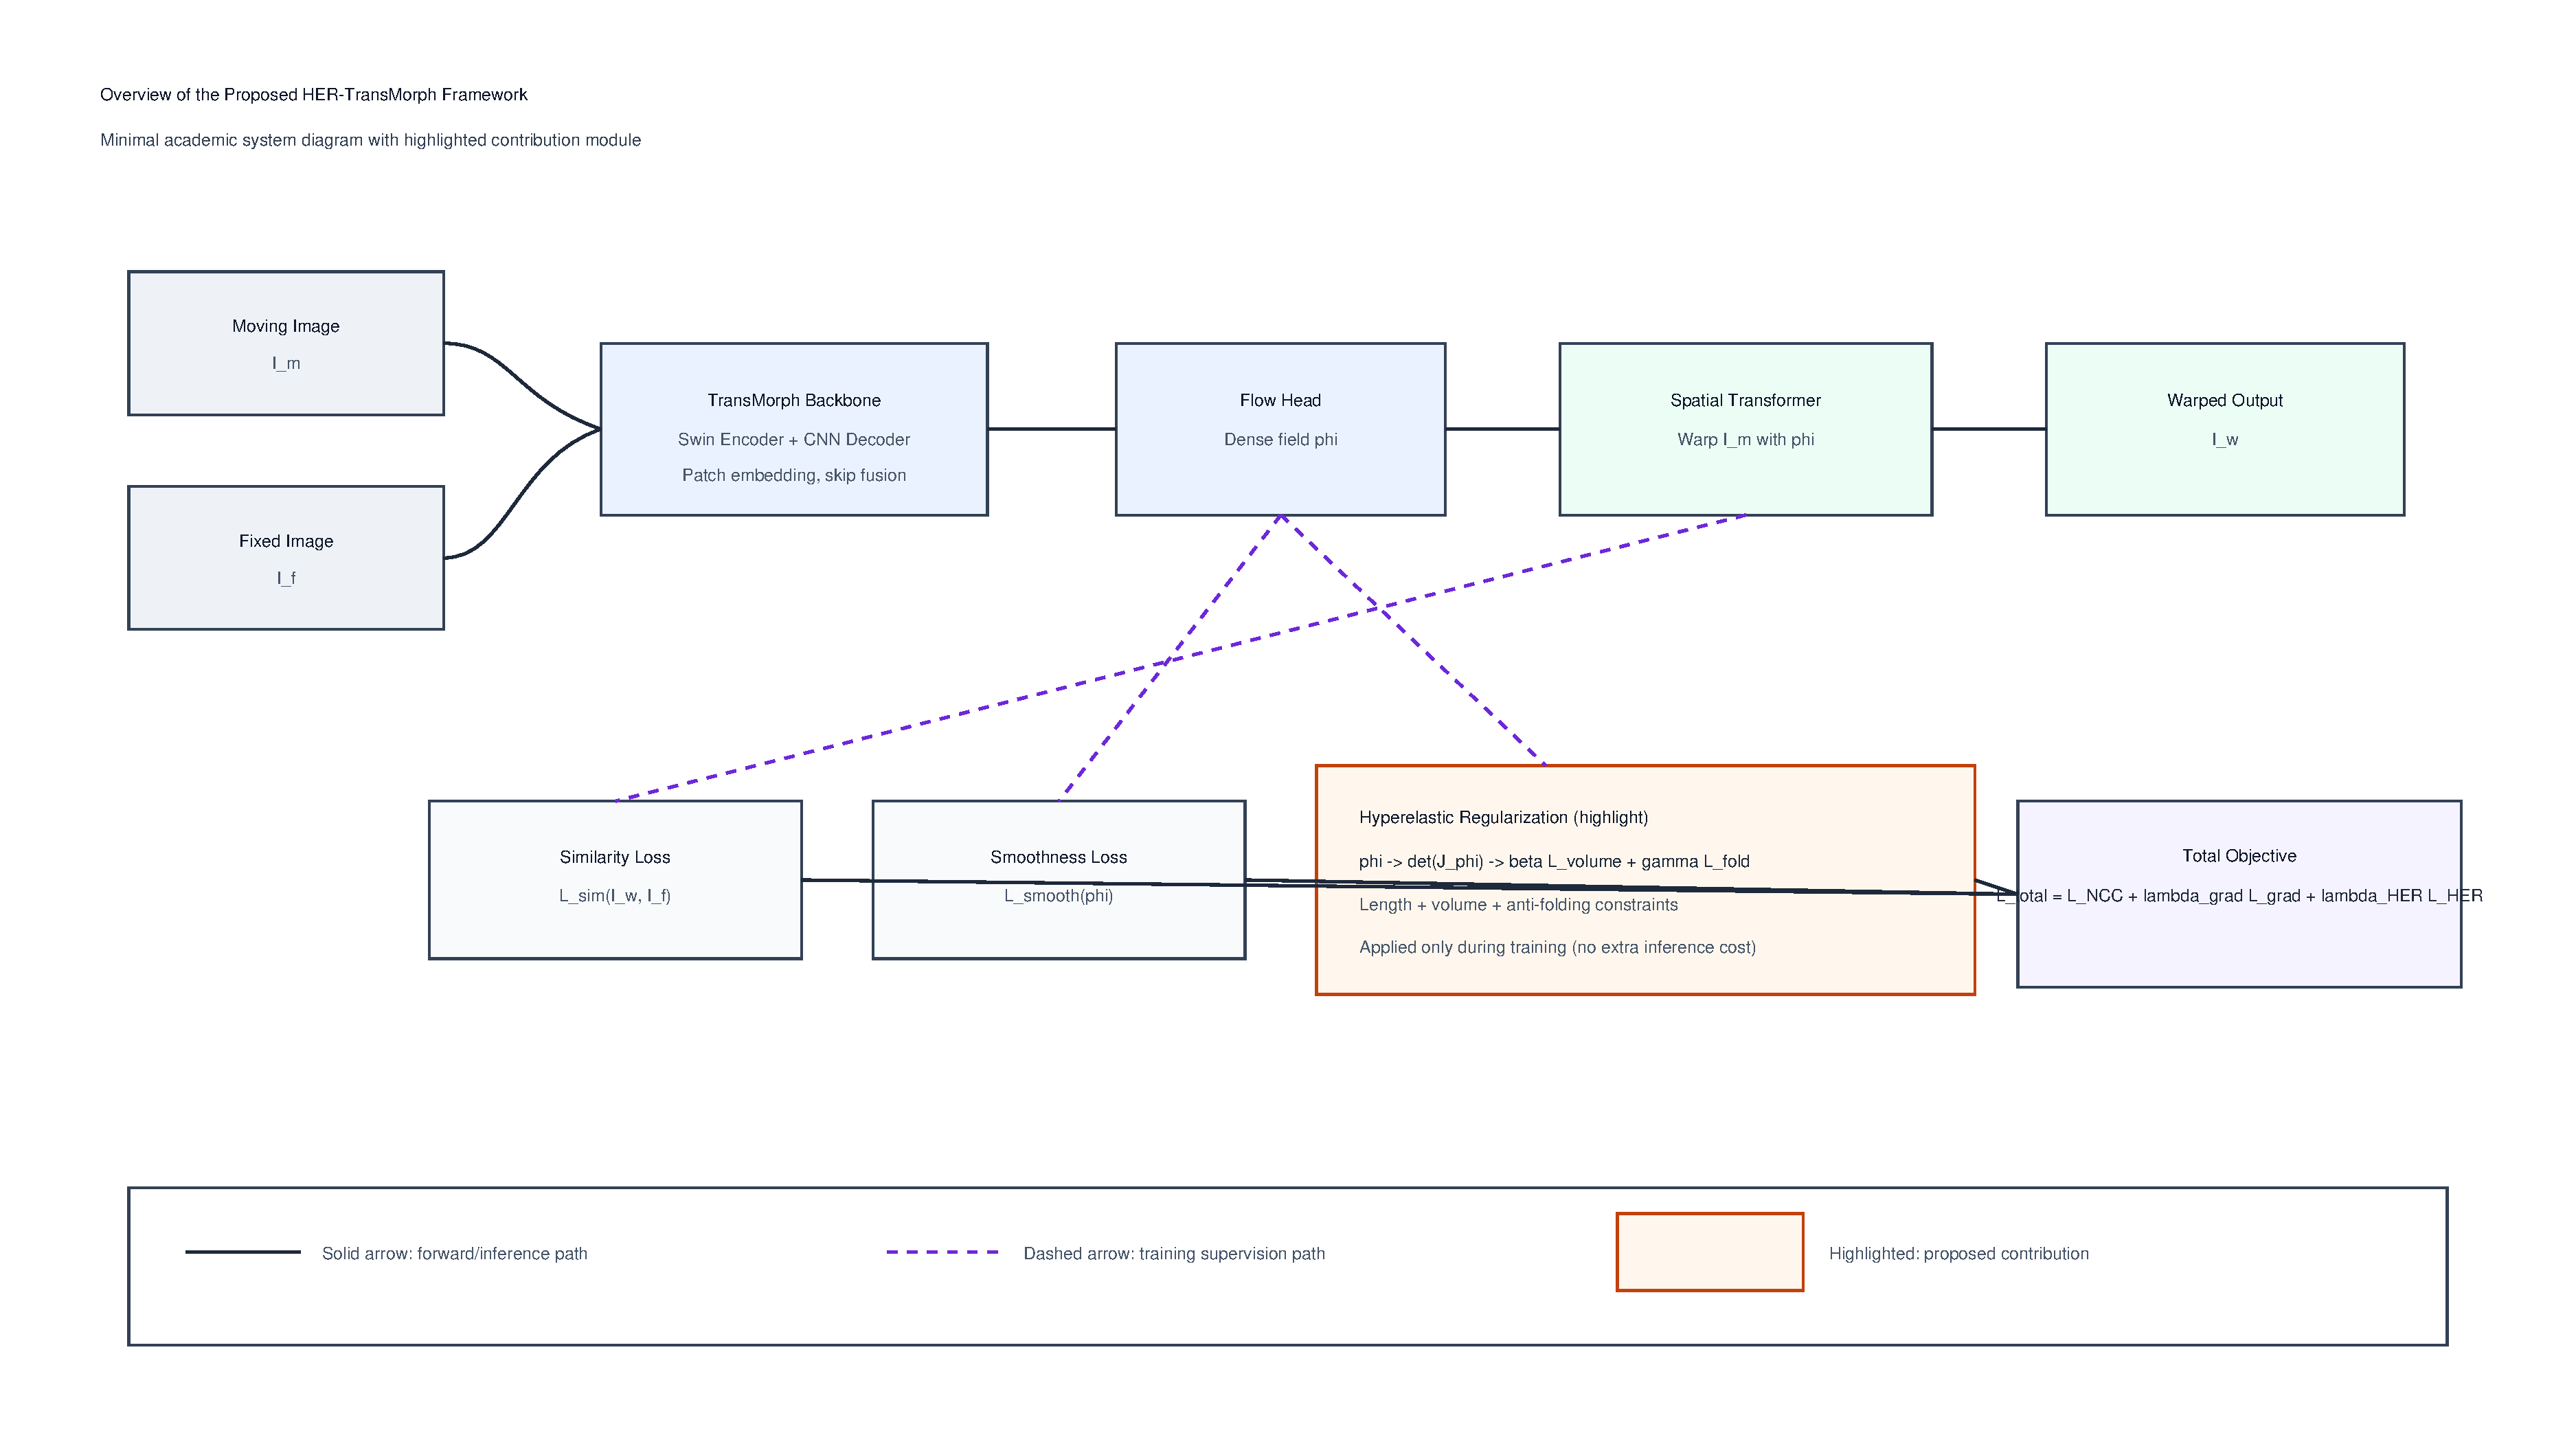
\includegraphics[width=0.96\textwidth]{figures/fig1_framework_figma.pdf}
\caption{Overview of the proposed HER-TransMorph framework. The main inference path follows the original registration pipeline, while the highlighted hyperelastic term \(L_{\mathrm{HER}}=\beta L_{\mathrm{volume}}+\gamma L_{\mathrm{fold}}\) is injected only during training. This design improves deformation plausibility without additional inference cost.\label{fig1}}
\end{figure}

% TODO Stage B: regenerate from real saved fields and subject IDs.
\begin{figure}[H]
\centering
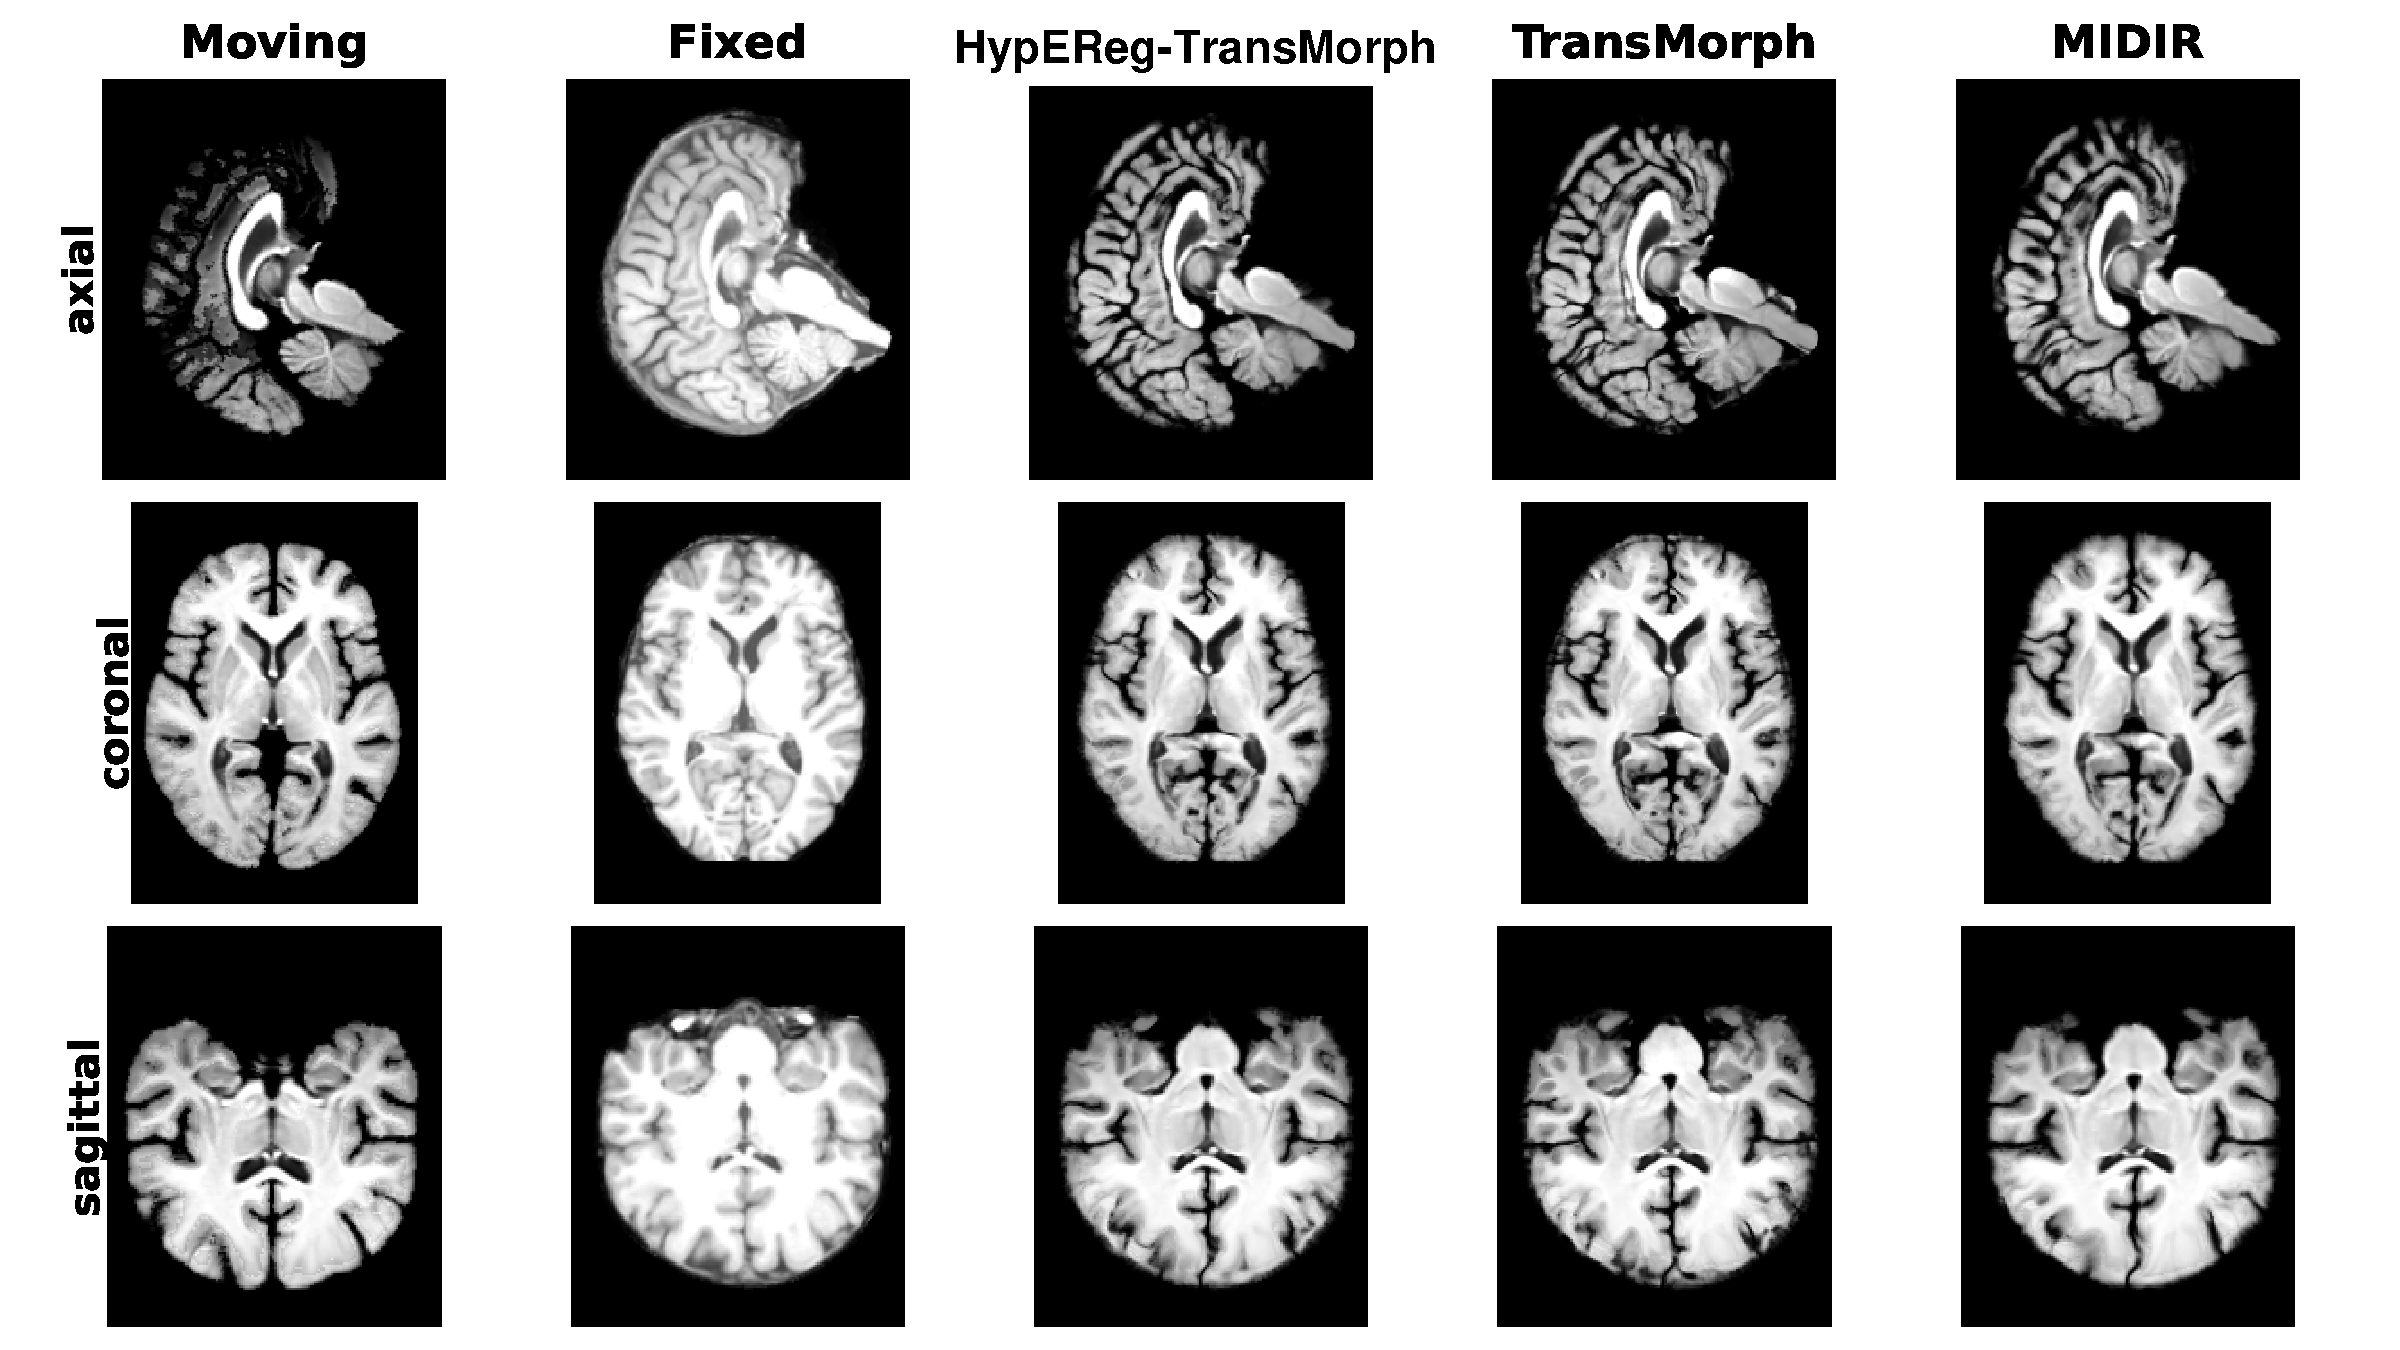
\includegraphics[width=0.96\textwidth]{figures/fig2_qualitative.pdf}
\caption{Qualitative registration comparisons on representative IXI and OASIS subjects. \PH{figure regenerated in Stage B from saved deformation fields}.\label{fig2}}
\end{figure}

% TODO Stage B: regenerate from real deformation grids.
\begin{figure}[H]
\centering
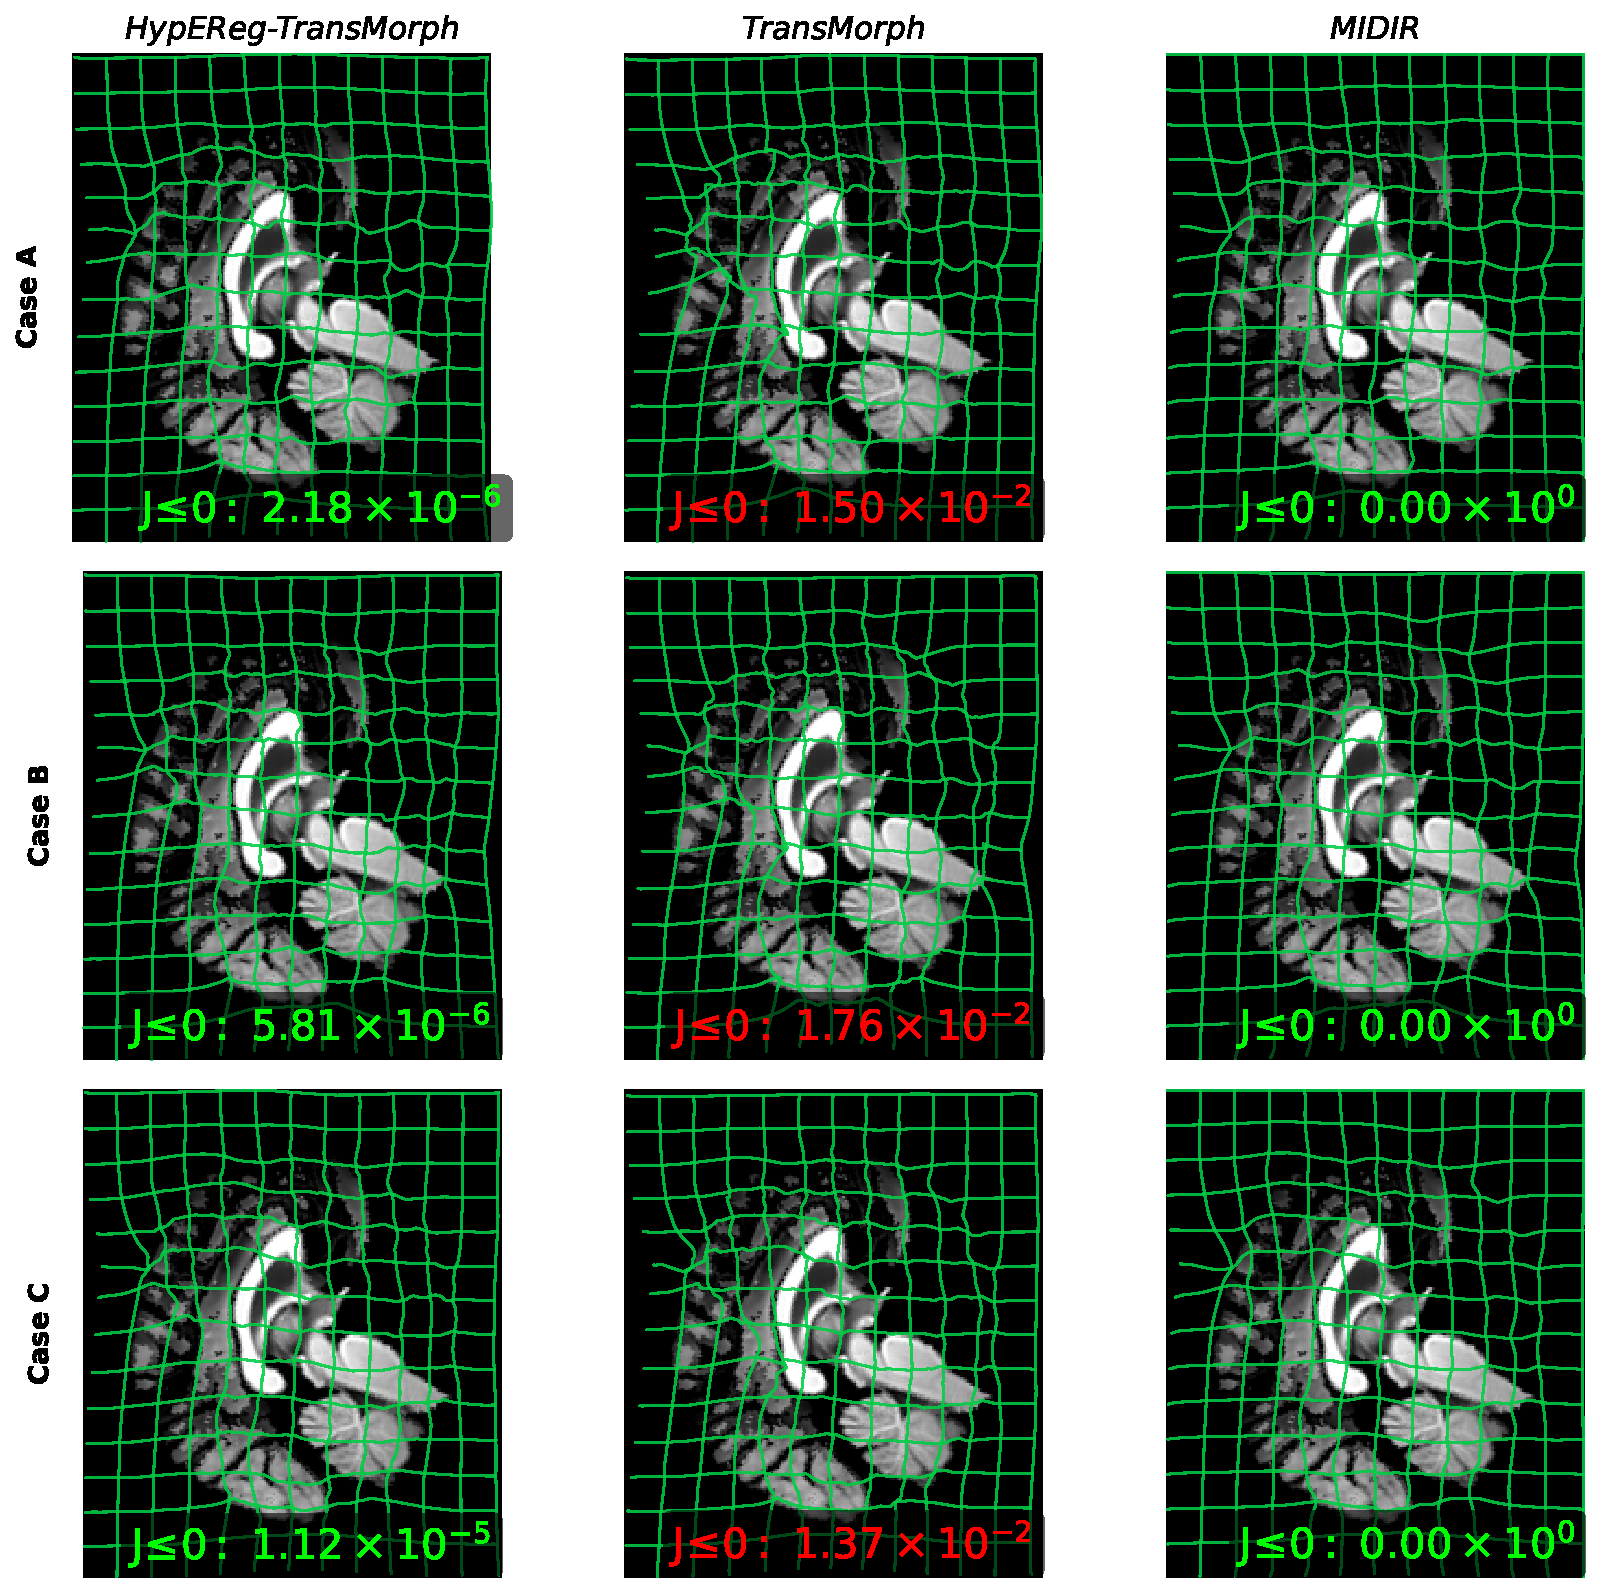
\includegraphics[width=0.96\textwidth]{figures/fig3_gridwarp.pdf}
\caption{Deformation grid visualization for competing methods, highlighting fold-free behavior in HER-TransMorph. \PH{figure regenerated in Stage B from saved deformation fields}.\label{fig3}}
\end{figure}

% TODO Stage B: regenerate from real Jacobian maps and histograms.
\begin{figure}[H]
\centering
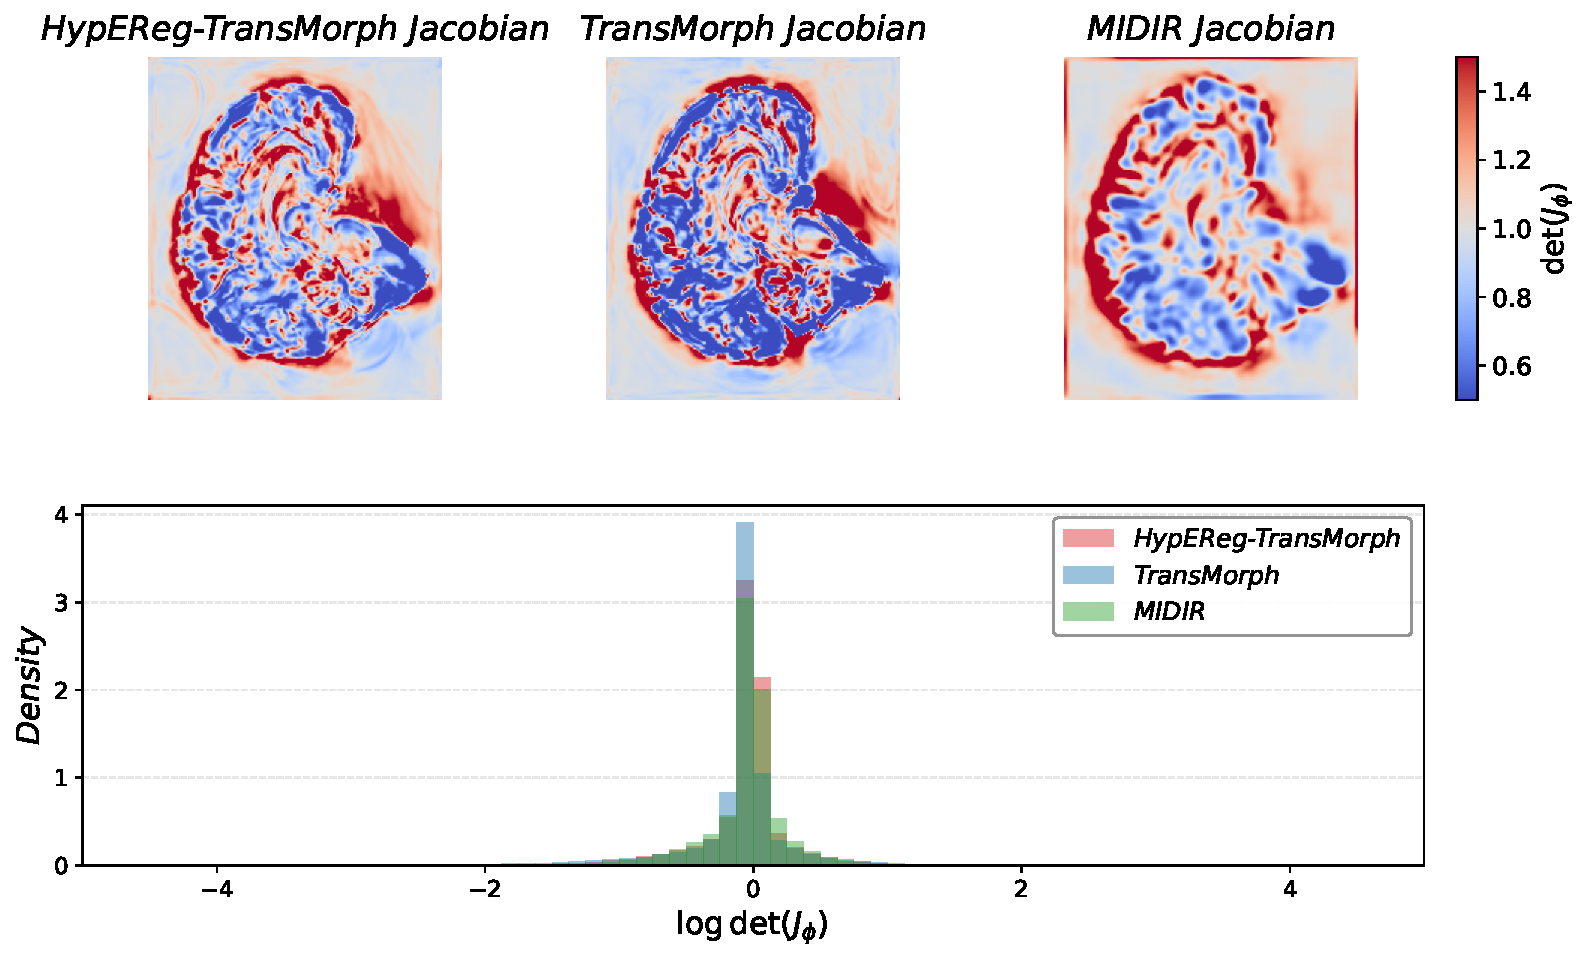
\includegraphics[width=0.96\textwidth]{figures/fig4_jacobian.pdf}
\caption{Jacobian determinant heatmaps and log\(|J|\) histograms for HER-TransMorph and baseline models. \PH{figure regenerated in Stage B from saved deformation fields}.\label{fig4}}
\end{figure}

% TODO Stage B: regenerate with IXI+OASIS dual panel metrics.
\begin{figure}[H]
\centering
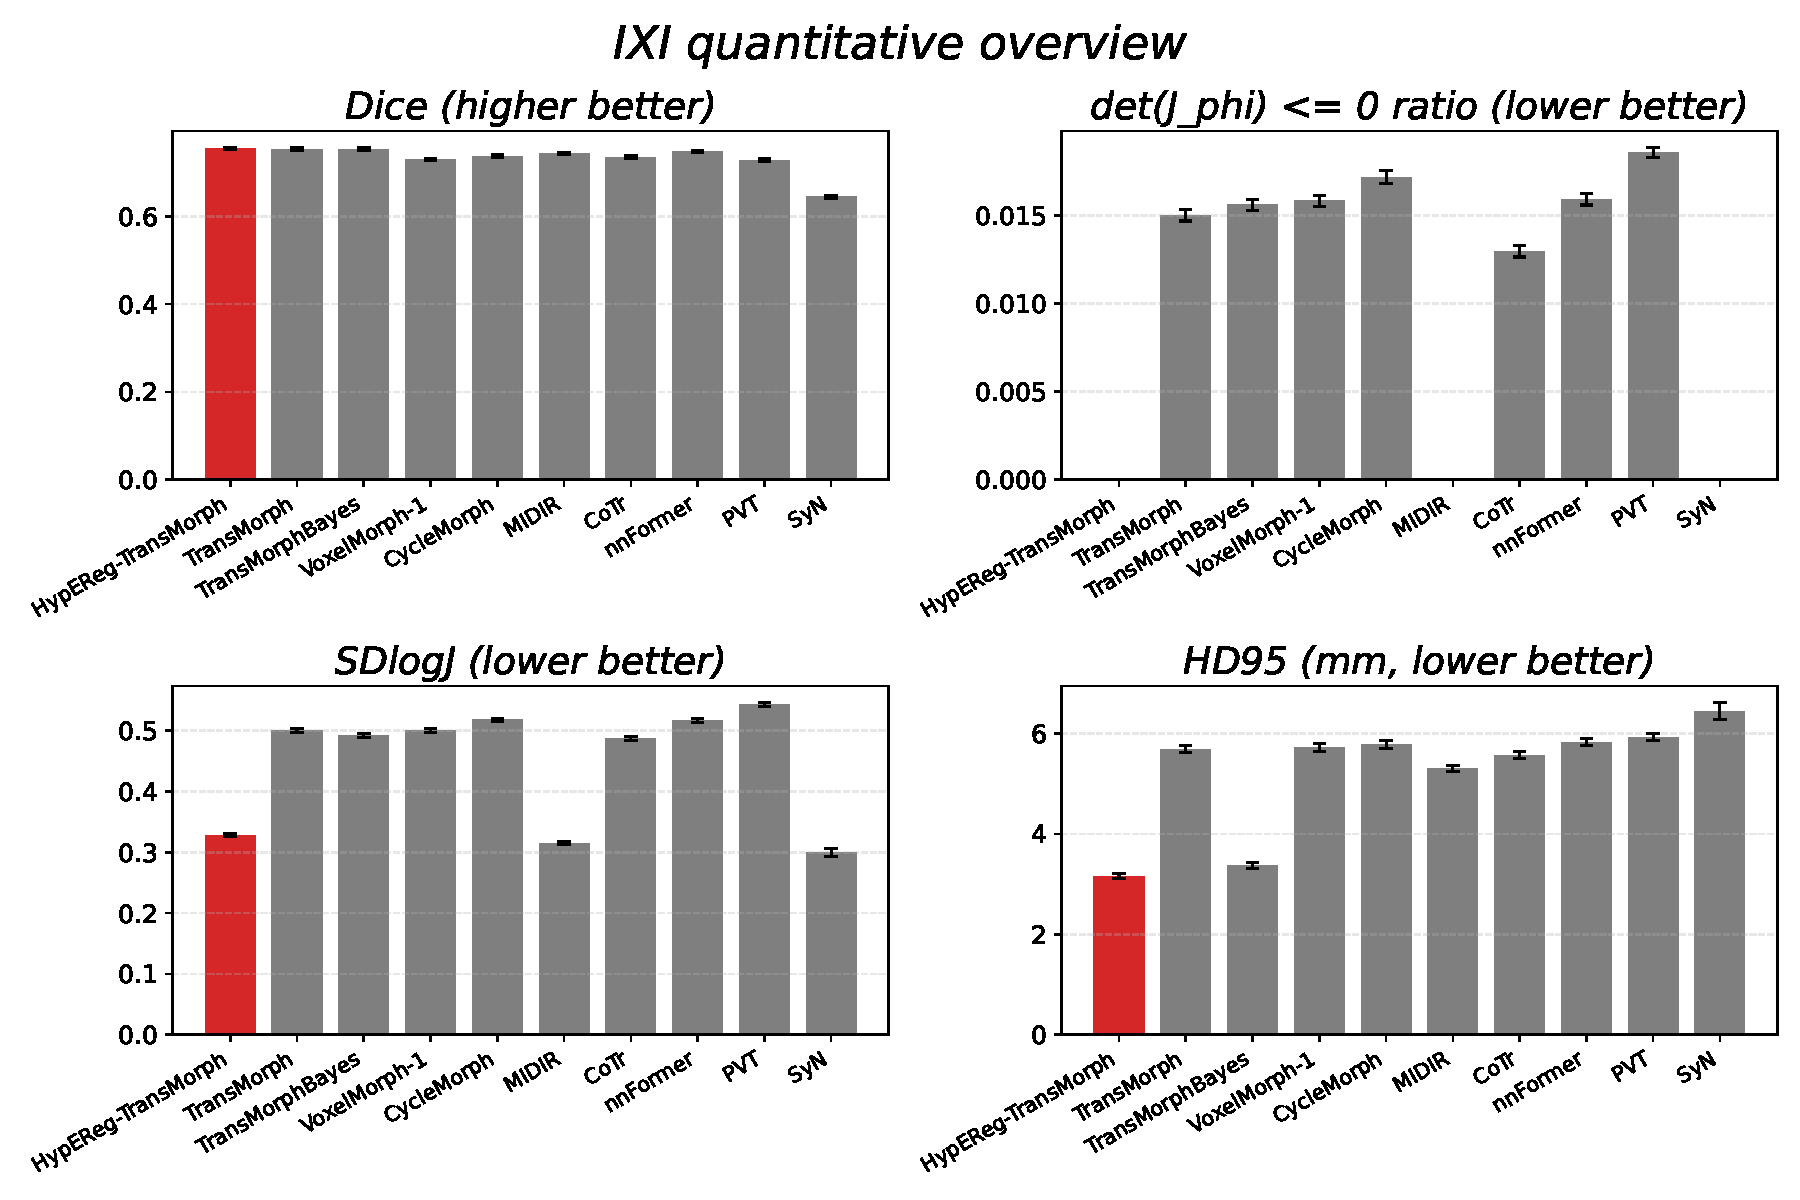
\includegraphics[width=0.99\textwidth]{figures/fig5_metrics.pdf}
\caption{Consolidated metric overview across selected methods (Dice, non\_jac, SDlogJ, bending energy, and runtime). \PH{figure regenerated in Stage B from IXI+OASIS panel data}.\label{fig5}}
\end{figure}

%%%%%%%%%%%%%%%%%%%%%%%%%%%%%%%%%%%%%%%%%%
\section{Discussion}

This work is positioned as a deformation-quality improvement study rather than a pure overlap-accuracy competition. The key result is that HER-TransMorph improves topology-preserving behavior (lower non\_jac and SDlogJ) while maintaining comparable Dice/HD95/ASSD to strong Transformer baselines. This trade-off is practically meaningful for downstream morphometric tasks that are sensitive to local folding artifacts.

The observed performance pattern suggests that adding physically motivated regularization to Transformer-based registration can constrain unrealistic local volume changes without substantially degrading alignment fidelity. In clinical and research workflows, this is relevant for Jacobian-based analyses, longitudinal disease progression studies, and atlas-based quantification where deformation plausibility matters beyond overlap scores.

The CNN/B-spline baseline MIDIR also achieves zero non-positive Jacobian ratio on IXI, with SDlogJ (0.3148) marginally lower than HER-TransMorph (0.3280). The two methods reach comparable regularity through different routes: MIDIR enforces smoothness implicitly via B-spline parameterization, while HER-TransMorph enforces regularity explicitly through differentiable hyperelastic penalties on dense flow. HER is plug-in to dense-flow backbones without changing parameterization, and preserves overlap expressivity (Dice 0.7537 vs.\ 0.7423 for MIDIR on IXI). Cross-dataset evidence on OASIS is summarized as \PH{OASIS MIDIR-vs-HER discussion pending Stage B}.

The OASIS inter-subject regime produces larger anatomical displacements than IXI atlas-to-subject. HER-TransMorph maintains a non-positive Jacobian ratio of \PH{HER non\_jac OASIS} under this harder regime versus \PH{TM-unsup non\_jac OASIS} for the unsupervised TransMorph comparator, with paired Wilcoxon + BH-FDR significance at \(q<\PH{OASIS q-value}\). The consistency of topology gains across two cohorts and protocols supports the generality of the hyperelastic-regularization mechanism.

Several limitations should be acknowledged. First, this manuscript retains a single training seed; multi-seed confidence intervals are future work. Second, a per-term ablation isolating \(\mathcal{L}_{\mathrm{length}}\), \(\mathcal{L}_{\mathrm{volume}}\), and \(\mathcal{L}_{\mathrm{fold}}\) was not rerun under the final operating-point pipeline; instead, cross-dataset OASIS validation is used as the main generalization check. Third, although IXI and OASIS cover two protocols, the study is still limited to structural brain MRI and does not yet include pathology-rich or multi-modal settings. Fourth, sensitivity sweeps for \(\beta\) and \(\gamma\) were not performed, and \(\alpha=0\) is a deliberate operating-point choice. Fifth, software-stack reproducibility against a stable PyTorch release is tracked as \PH{stable-PyTorch verification pending Stage B}.

Future work will extend HER to multi-modal registration, pathology-rich cohorts, and uncertainty-aware registration frameworks. Another direction is adaptive hyperelastic weighting to better balance local accuracy and topology constraints under heterogeneous anatomical deformations.

%%%%%%%%%%%%%%%%%%%%%%%%%%%%%%%%%%%%%%%%%%
\section{Conclusions}

HER-TransMorph introduces hyperelastic constraints into Transformer-based deformable registration and delivers topology-preserving deformations with competitive registration accuracy. Across the unified IXI evaluation protocol, HER-TransMorph demonstrates marked gains in deformation regularity metrics while maintaining strong overlap performance. These results support HER as a practical registration design for anatomically reliable brain MRI alignment.

This draft is Stage-A complete and will be finalized for submission after Stage-B replacement of all \(\PH{...}\) entries with computed results.

%%%%%%%%%%%%%%%%%%%%%%%%%%%%%%%%%%%%%%%%%%
\vspace{6pt} 

%%%%%%%%%%%%%%%%%%%%%%%%%%%%%%%%%%%%%%%%%%
%% optional
\supplementary{Supplementary materials include: Table S1 (full metric panel including intensity and efficiency metrics), Table S2 (paired Wilcoxon + BH-FDR significance matrix), additional qualitative registration and Jacobian visualizations, and implementation details. Files will be uploaded as \texttt{supplementary.pdf} and companion data archives.}

% Only for journal Methods and Protocols:
% If you wish to submit a video article, please do so with any other supplementary material.
% \supplementary{The following supporting information can be downloaded at: \linksupplementary{s1}, Figure S1: title; Table S1: title; Video S1: title. A supporting video article is available at doi: link.}

% Only used for preprtints:
% \supplementary{The following supporting information can be downloaded at the website of this paper posted on \href{https://www.preprints.org/}{Preprints.org}.}

% Only for journal Hardware:
% If you wish to submit a video article, please do so with any other supplementary material.
% \supplementary{The following supporting information can be downloaded at: \linksupplementary{s1}, Figure S1: title; Table S1: title; Video S1: title.\vspace{6pt}\\
%\begin{tabularx}{\textwidth}{lll}
%\toprule
%\textbf{Name} & \textbf{Type} & \textbf{Description} \\
%\midrule
%S1 & Python script (.py) & Script of python source code used in XX \\
%S2 & Text (.txt) & Script of modelling code used to make Figure X \\
%S3 & Text (.txt) & Raw data from experiment X \\
%S4 & Video (.mp4) & Video demonstrating the hardware in use \\
%... & ... & ... \\
%\bottomrule
%\end{tabularx}
%}

%%%%%%%%%%%%%%%%%%%%%%%%%%%%%%%%%%%%%%%%%%
\authorcontributions{Conceptualization, A.O.; methodology, A.O. and A.T.; software, A.O.; validation, A.O. and C.A.; formal analysis, A.O.; investigation, A.O.; data curation, A.O.; writing---original draft preparation, A.O.; writing---review and editing, A.O., A.T., and C.A.; visualization, A.O.; supervision, C.A.; project administration, C.A. All authors have read and agreed to the published version of the manuscript.}

\funding{This research received no external funding.}

\institutionalreview{Ethical review and approval were waived for this study because only publicly available, anonymized IXI data were used.}

\informedconsent{Patient consent was waived because this study used anonymized publicly available data.}

\dataavailability{The IXI dataset used in this study is publicly available at \url{https://brain-development.org/ixi-dataset/}. Code and evaluation scripts are available at \url{https://github.com/TBD/HER-TransMorph}. Derived evaluation tables and figures are provided in the supplementary materials.} 

%\durcstatement{Current research is limited to the [please insert a specific academic field, e.g., XXX], which is beneficial [share benefits and/or primary use] and does not pose a threat to public health or national security. Authors acknowledge the dual-use potential of the research involving xxx and confirm that all necessary precautions have been taken to prevent potential misuse. As an ethical responsibility, authors strictly adhere to relevant national and international laws about DURC. Authors advocate for responsible deployment, ethical considerations, regulatory compliance, and transparent reporting to mitigate misuse risks and foster beneficial outcomes.}

% Only for journal Nursing Reports
%\publicinvolvement{Please describe how the public (patients, consumers, carers) were involved in the research. Consider reporting against the GRIPP2 (Guidance for Reporting Involvement of Patients and the Public) checklist. If the public were not involved in any aspect of the research add: ``No public involvement in any aspect of this research''.}
%
%% Only for journal Nursing Reports
%\guidelinesstandards{Please add a statement indicating which reporting guideline was used when drafting the report. For example, ``This manuscript was drafted against the XXX (the full name of reporting guidelines and citation) for XXX (type of research) research''. A complete list of reporting guidelines can be accessed via the equator network: \url{https://www.equator-network.org/}.}
%
%% Only for journal Nursing Reports
%\useofartificialintelligence{Please describe in detail any and all uses of artificial intelligence (AI) or AI-assisted tools used in the preparation of the manuscript. This may include, but is not limited to, language translation, language editing and grammar, or generating text. Alternatively, please state that “AI or AI-assisted tools were not used in drafting any aspect of this manuscript”.}

\acknowledgments{The authors thank the maintainers of open-source registration baselines and the IXI data contributors.}

\conflictsofinterest{The authors declare no conflicts of interest.}

%%%%%%%%%%%%%%%%%%%%%%%%%%%%%%%%%%%%%%%%%%
%% Optional

%% Only for journal Encyclopedia
%\entrylink{The Link to this entry published on the encyclopedia platform.}

\abbreviations{Abbreviations}{
The following abbreviations are used in this manuscript:
\\
\noindent
\begin{tabular}{@{}ll}
HER & Hyperelastic Regularization\\
MRI & Magnetic Resonance Imaging\\
HD95 & 95th percentile Hausdorff Distance\\
ASSD & Average Symmetric Surface Distance\\
NCC & Normalized Cross-Correlation\\
LNCC & Local Normalized Cross-Correlation\\
SDlogJ & Standard Deviation of Log Jacobian Determinant\\
IXI & Information eXtraction from Images dataset\\
GPU & Graphics Processing Unit
\end{tabular}
}

%%%%%%%%%%%%%%%%%%%%%%%%%%%%%%%%%%%%%%%%%%
%% Optional
\appendixtitles{no} % Leave argument "no" if all appendix headings stay EMPTY (then no dot is printed after "Appendix A"). If the appendix sections contain a heading then change the argument to "yes".
\appendixstart
\appendix
\section[\appendixname~\thesection]{Supplementary Experimental Details}
\subsection[\appendixname~\thesubsection]{Model and Environment Configuration}
This appendix summarizes implementation details required for reproducibility:
\begin{itemize}
\item Framework and package versions: Python 3.12.10; PyTorch 2.12.0.dev20260408+cu128 (current runs); planned stable verification on PyTorch 2.5.x + CUDA 12.4 (\PH{status pending Stage B}); antspyx 0.6.3; SimpleITK 2.5.3.
\item Hardware configuration: NVIDIA RTX PRO 6000 Blackwell Workstation Edition (97,887 MiB VRAM), driver 591.86; CPU/RAM configuration should be reported from the submission host inventory. Peak-memory audits from available \texttt{IXI/Eval\_Results/*/per\_case.csv} files indicate a single-GPU run profile for deep models, while classical baselines remain \PH{pending full rerun verification}.
\item Checkpoint list and paths: see \texttt{IXI/eval\_configs.yaml} model adapters and associated checkpoint manifests in \texttt{IXI/Eval\_Results/*/meta.json}.
\item Inference command templates and evaluation flags: \texttt{python IXI/run\_full\_eval.py --config IXI/eval\_configs.yaml --no-aggregate}; metrics/label settings are defined in \texttt{IXI/eval\_configs.yaml}.
\end{itemize}

\section[\appendixname~\thesection]{Extended Quantitative Tables}
\begin{table}[H]
\caption{Supplementary full metric panel (updated after Stage-B export completion).\label{tab5}}
\begin{tabularx}{\textwidth}{lccc}
\toprule
\textbf{Metric Group} & \textbf{HER-TransMorph} & \textbf{Best Baseline} & \textbf{q-value}\\
\midrule
Intensity metrics (NCC/LNCC/MI/NMI/SSIM/PSNR) & 0.9539/0.2738/0.7317/1.2812/0.9106/26.4485 & 0.9639/0.3069/0.7856/1.3040/0.9295/27.2355 & N/A (pending full paired FDR export)\\
Jacobian quantiles (\(J_{p01},J_{p50},J_{p99}\)) & 0.2754 / 0.9775 / 2.1284 & -0.0871 / 0.9334 / 2.5926 & N/A (pending full paired FDR export)\\
Efficiency (runtime/peak memory) & 0.2034 s / 10.635 GB & 3.5372 s / 16.088 GB & N/A (observation metric)\\
\bottomrule
\end{tabularx}
\end{table}

%%%%%%%%%%%%%%%%%%%%%%%%%%%%%%%%%%%%%%%%%%
%\isPreprints{}{% This command is only used for ``preprints''.
\begin{adjustwidth}{-\extralength}{0cm}
%} % If the paper is ``preprints'', please uncomment this parenthesis.
%\printendnotes[custom] % Un-comment to print a list of endnotes

\reftitle{References}

% Please provide either the correct journal abbreviation (e.g. according to the “List of Title Word Abbreviations” http://www.issn.org/services/online-services/access-to-the-ltwa/) or the full name of the journal.
% Citations and References in Supplementary files are permitted provided that they also appear in the reference list here. 

%=====================================
% References, variant A: external bibliography
%=====================================
\bibliography{refs}

%=====================================
% References, variant B: internal bibliography
%=====================================
\iffalse

% ACS format
\isAPAandChicago{}{%
\begin{thebibliography}{999}
% Reference 1
\bibitem[Author1(year)]{ref-journal}
Author~1, T. The title of the cited article. {\em Journal Abbreviation} {\bf 2008}, {\em 10}, 142--149.
% Reference 2
\bibitem[Author2(year)]{ref-book1}
Author~2, L. The title of the cited contribution. In {\em The Book Title}; Editor 1, F., Editor 2, A., Eds.; Publishing House: City, Country, 2007; pp. 32--58.
% Reference 3
\bibitem[Author1 and Author2 (year)]{ref-book2}
Author 1, A.; Author 2, B. \textit{Book Title}, 3rd ed.; Publisher: Publisher Location, Country, 2008; pp. 154--196.
% Reference 4
\bibitem[Author4(year)]{ref-unpublish}
Author 1, A.B.; Author 2, C. Title of Unpublished Work. \textit{Abbreviated Journal Name} year, \textit{phrase indicating stage of publication (submitted; accepted; in press)}.
% Reference 5
\bibitem[Author8(year)]{ref-url}
Title of Site. Available online: URL (accessed on Day Month Year).
% Reference 6
\bibitem[Author6(year)]{ref-proceeding}
Author 1, A.B.; Author 2, C.D.; Author 3, E.F. Title of presentation. In Proceedings of the Name of the Conference, Location of Conference, Country, Date of Conference (Day Month Year); Abstract Number (optional), Pagination (optional).
% Reference 7
\bibitem[Author7(year)]{ref-thesis}
Author 1, A.B. Title of Thesis. Level of Thesis, Degree-Granting University, Location of University, Date of Completion.
\end{thebibliography}
}

% Chicago format (Used for journal: arts, genealogy, histories, humanities, jintelligence, laws, literature, religions, risks, socsci)
\isChicagoStyle{%
\begin{thebibliography}{999}
% Reference 1
\bibitem[Aranceta-Bartrina(1999a)]{ref-journal}
Aranceta-Bartrina, Javier. 1999a. Title of the cited article. \textit{Journal Title} 6: 100--10.
% Reference 2
\bibitem[Aranceta-Bartrina(1999b)]{ref-book1}
Aranceta-Bartrina, Javier. 1999b. Title of the chapter. In \textit{Book Title}, 2nd ed. Edited by Editor 1 and Editor 2. Publication place: Publisher, vol. 3, pp. 54–96.
% Reference 3
\bibitem[Baranwal and Munteanu {[1921]}(1955)]{ref-book2}
Baranwal, Ajay K., and Costea Munteanu. 1955. \textit{Book Title}. Publication place: Publisher, pp. 154--96. First published 1921 (op-tional).
% Reference 4
\bibitem[Berry and Smith(1999)]{ref-thesis}
Berry, Evan, and Amy M. Smith. 1999. Title of Thesis. Level of Thesis, Degree-Granting University, City, Country. Identifi-cation information (if available).
% Reference 5
\bibitem[Cojocaru et al.(1999)]{ref-unpublish}
Cojocaru, Ludmila, Dragos Constatin Sanda, and Eun Kyeong Yun. 1999. Title of Unpublished Work. \textit{Journal Title}, phrase indicating stage of publication.
% Reference 6
\bibitem[Driver et al.(2000)]{ref-proceeding}
Driver, John P., Steffen Rohrs, and Sean Meighoo. 2000. Title of Presentation. In \textit{Title of the Collected Work} (if available). Paper presented at Name of the Conference, Location of Conference, Date of Conference.
% Reference 7
\bibitem[Harwood(2008)]{ref-url}
Harwood, John. 2008. Title of the cited article. Available online: URL (accessed on Day Month Year).
\end{thebibliography}
}{}

% APA format (Used for journal: admsci, behavsci, businesses, econometrics, economies, education, ejihpe, games, humans, ijfs, journalmedia, jrfm, languages, psycholint, publications, tourismhosp, youth)
\isAPAStyle{%
\begin{thebibliography}{999}
% Reference 1
\bibitem[\protect\citeauthoryear{Azikiwe \BBA\ Bello}{{2020a}}]{ref-journal}
Azikiwe, H., \& Bello, A. (2020a). Title of the cited article. \textit{Journal Title}, \textit{Volume}(Issue), 
Firstpage--Lastpage/Article Number.
% Reference 2
\bibitem[\protect\citeauthoryear{Azikiwe \BBA\ Bello}{{2020b}}]{ref-book1}
Azikiwe, H., \& Bello, A. (2020b). \textit{Book title}. Publisher Name.
% Reference 3
\bibitem[Davison(1623/2019)]{ref-book2}
Davison, T. E. (2019). Title of the book chapter. In A. A. Editor (Ed.), \textit{Title of the book: Subtitle} 
(pp. Firstpage--Lastpage). Publisher Name. (Original work published 1623) (Optional).
% Reference 4
\bibitem[Fistek et al.(2017)]{ref-proceeding}
Fistek, A., Jester, E., \& Sonnenberg, K. (2017, Month Day). Title of contribution [Type of contribution]. Conference Name, Conference City, Conference Country.
% Reference 5
\bibitem[Hutcheson(2012)]{ref-thesis}
Hutcheson, V. H. (2012). \textit{Title of the thesis} [XX Thesis, Name of Institution Awarding the Degree].
% Reference 6
\bibitem[Lippincott \& Poindexter(2019)]{ref-unpublish}
Lippincott, T., \& Poindexter, E. K. (2019). \textit{Title of the unpublished manuscript} [Unpublished manuscript/Manuscript in prepara-tion/Manuscript submitted for publication]. Department Name, Institution Name.
% Reference 7
\bibitem[Harwood(2008)]{ref-url}
Harwood, J. (2008). \textit{Title of the cited article}. Available online: URL (accessed on Day Month Year).
\end{thebibliography}
}{}
\fi

% If authors have biography, please use the format below
%\section*{Short Biography of Authors}
%\bio
%{\raisebox{-0.35cm}{\includegraphics[width=3.5cm,height=5.3cm,clip,keepaspectratio]{Definitions/author1.pdf}}}
%{\textbf{Firstname Lastname} Biography of first author}
%
%\bio
%{\raisebox{-0.35cm}{\includegraphics[width=3.5cm,height=5.3cm,clip,keepaspectratio]{Definitions/author2.jpg}}}
%{\textbf{Firstname Lastname} Biography of second author}

% For the MDPI journals use author-date citation, please follow the formatting guidelines on http://www.mdpi.com/authors/references
% To cite two works by the same author: \citeauthor{ref-journal-1a} (\citeyear{ref-journal-1a}, \citeyear{ref-journal-1b}). This produces: Whittaker (1967, 1975)
% To cite two works by the same author with specific pages: \citeauthor{ref-journal-3a} (\citeyear{ref-journal-3a}, p. 328; \citeyear{ref-journal-3b}, p.475). This produces: Wong (1999, p. 328; 2000, p. 475)

%%%%%%%%%%%%%%%%%%%%%%%%%%%%%%%%%%%%%%%%%%
%% for journal Sci
%\reviewreports{\\
%Reviewer 1 comments and authors’ response\\
%Reviewer 2 comments and authors’ response\\
%Reviewer 3 comments and authors’ response
%}
%%%%%%%%%%%%%%%%%%%%%%%%%%%%%%%%%%%%%%%%%%
\PublishersNote{}
%\isPreprints{}{% This command is only used for ``preprints''.
\end{adjustwidth}
%} % If the paper is ``preprints'', please uncomment this parenthesis.
\end{document}

